% Created 2022-11-24 Thu 22:24
\documentclass[9pt, b5paper]{article}
\usepackage{xeCJK}
\usepackage{minted}
\usepackage[T1]{fontenc}
\usepackage[scaled]{beraserif}
\usepackage[scaled]{berasans}
\usepackage[scaled]{beramono}
\usepackage{graphicx}
\usepackage{xcolor}
\usepackage{multirow}
\usepackage{multicol}
\usepackage{float}
\usepackage{textcomp}
\usepackage{algorithm}
\usepackage{algorithmic}
\usepackage{latexsym}
\usepackage{natbib}
\usepackage{geometry}
\geometry{left=1.2cm,right=1.2cm,top=1.5cm,bottom=1.2cm}
\newminted{common-lisp}{fontsize=\footnotesize} 
\usepackage[xetex,colorlinks=true,CJKbookmarks=true,linkcolor=blue,urlcolor=blue,menucolor=blue]{hyperref}
\author{deepwaterooo}
\date{\today}
\title{Unity Export 导出到Android Studio再打包大致过程}
\hypersetup{
  pdfkeywords={},
  pdfsubject={},
  pdfcreator={Emacs 27.2 (Org mode 8.2.7c)}}
\begin{document}

\maketitle
\tableofcontents


\section{导出的unity项目文件大致是这样的}
\label{sec-1}
\begin{itemize}
\item 大致过程记一下,用作参考,原理还没有吃透,细节又比较多,容易忘记.作个笔记记一下,给自己用作参考
\end{itemize}

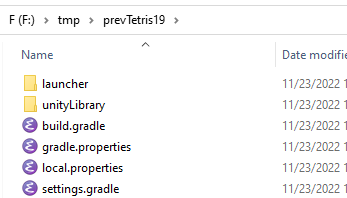
\includegraphics[width=.9\linewidth]{./pic/unityToAndroid_20221123_222322.png}
\begin{itemize}
\item 下面是2019年的版本可以打出两个文件夹,一个主工程,一个类库的导出包,2017年我用的版本打不出来,还需要想得再深一点多点儿,到可以按照这个笔记过程打包才行
\item 原始自己参考的项目是用2017版本的,当时没有吃透这里面的构建关系,当时以为只能用2017的unity和2017的Visual Studio才能开发.现在知道2019的版本能够导出自己可以调试的Android Studio项目,而unity 2017版本的导出来自己还仍不知道该如何从Android Studio打包,那么就暂时先用2019的版本,先试图打出在安卓设备上可运行的包,才能move on.
\end{itemize}
\section{Android创建、unity导入}
\label{sec-2}
\subsection{首先新建一个Android项目}
\label{sec-2-1}

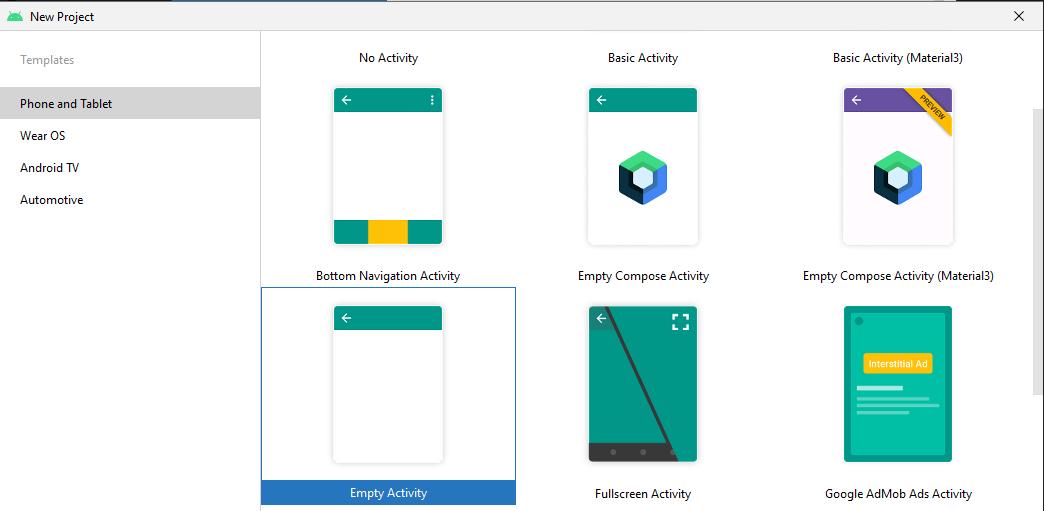
\includegraphics[width=.9\linewidth]{./pic/unityToAndroid_20221123_222542.png}
\begin{itemize}
\item 包名Package name跟unity的包名设置成一致,unity包名一般是 \textbf{com.unity3d.player} 。包名不一致的话,我试过也可以实现,但是在调用的时候要指明包,容易混淆,可能还有其他的一些问题,个人也不是很清楚。推荐保持一致,避免麻烦。Android项目名Name等随意。
\end{itemize}
\subsection{将unity项目以Module的方式导入Android}
\label{sec-2-2}

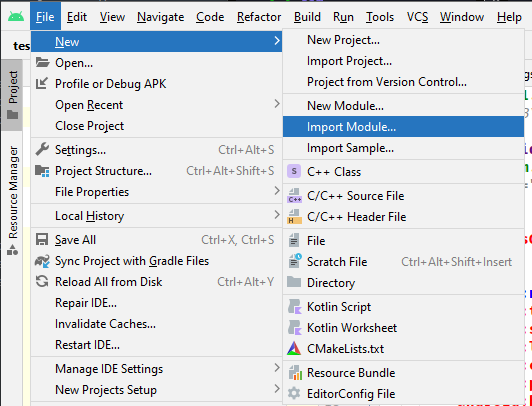
\includegraphics[width=.9\linewidth]{./pic/unityToAndroid_20221123_222637.png}

\subsection{选择unityLibrary导入。点击Finish}
\label{sec-2-3}

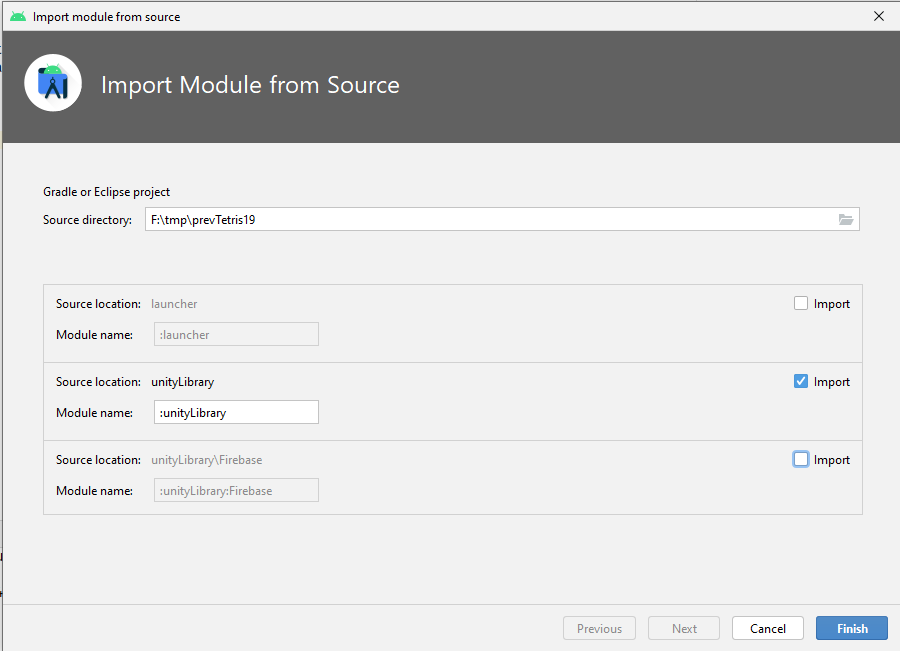
\includegraphics[width=.9\linewidth]{./pic/unityToAndroid_20221123_222720.png}
\subsection{导入之后,为Android添加unityLibrary的引用}
\label{sec-2-4}
\begin{itemize}
\item 左上角File——>Project Structure\ldots{}
\item 选择Dependencies  ——>  app ,然后点击右边这个加号 + ,选择第三个Moudule Dependency
\end{itemize}

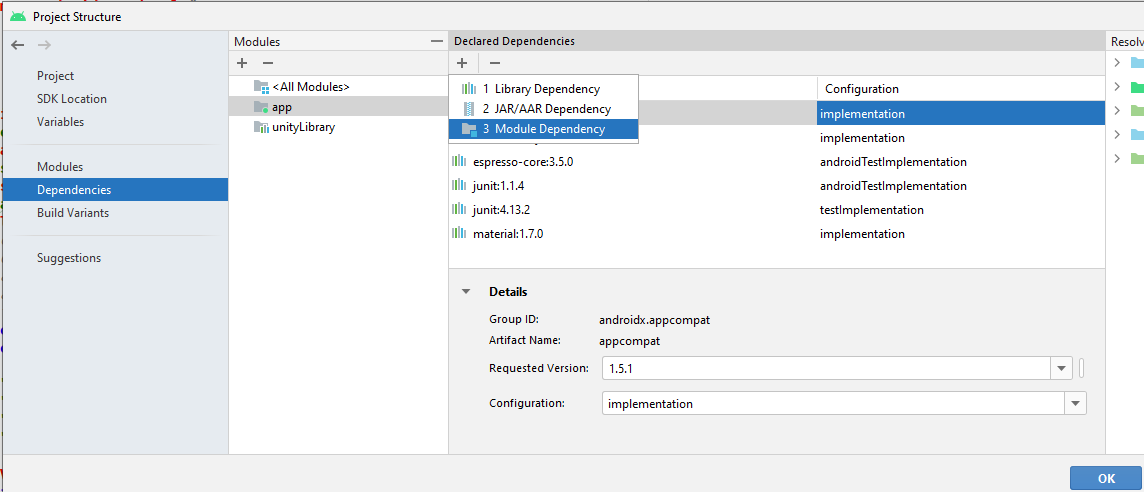
\includegraphics[width=.9\linewidth]{./pic/unityToAndroid_20221123_220755.png}
\begin{itemize}
\item 勾选刚刚导入的unity,点击OK。再点击上图的OK。
\end{itemize}

\subsection{配置 Android 以及 unity 的 build.gradle 文件}
\label{sec-2-5}
\begin{itemize}
\item 将SDK配置成当前Android版本可以运行。Android 以及unity的SDK确保要一样,不然会报错,比如这个minsdk。Build无误就算是导入完成了!

\item 这里作些简单的版本修改适配自己的手机,到项目可以构建成功为止.
\end{itemize}

\section{Android  启动运行 unity}
\label{sec-3}
\subsection{在unity的AndroidMainfest.xml文件}
\label{sec-3-1}
\begin{itemize}
\item 把<intent-filter>-->删掉或者注释掉,留着的话,当我们把程序运行到手机或者模拟机上时会有两个图标。
\item 其次是在<activity>里加入这行代码,实现多线程,避免在从unity返回Android时也将Android界面也结束了。
\begin{minted}[fontsize=\scriptsize,linenos=false]{xml}
android:process=":raadidcard"
\end{minted}
\end{itemize}

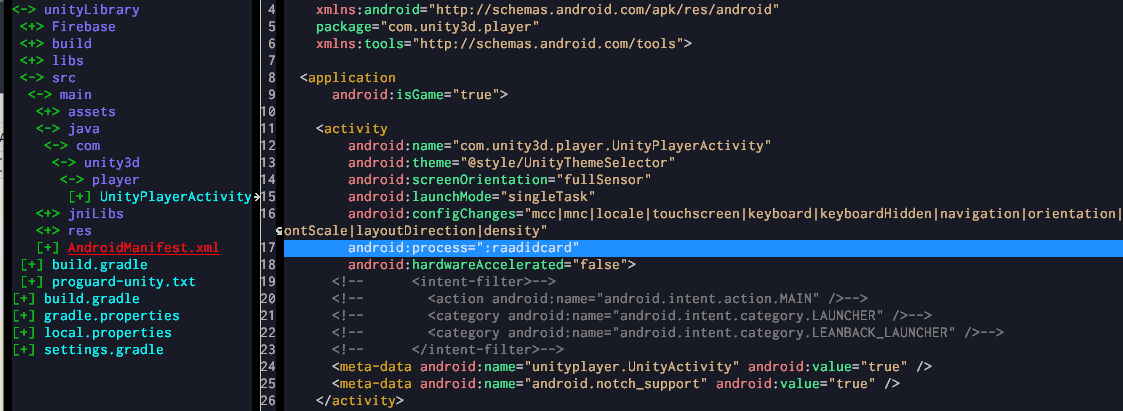
\includegraphics[width=.9\linewidth]{./pic/unityToAndroid_20221123_223227.png}
\subsection{在app的AndroidMainfest.xml文件里,在图中位置加入这两行代码:}
\label{sec-3-2}
\begin{minted}[fontsize=\scriptsize,linenos=false]{xml}
xmlns:tools="http://schemas.android.com/tools"

tools:replace="android:icon,android:theme,android:allowBackup"
\end{minted}
\begin{itemize}
\item 可以成片复制的代码如下:
\begin{minted}[fontsize=\scriptsize,linenos=false]{xml}
<?xml version="1.0" encoding="utf-8"?>
<manifest xmlns:android="http://schemas.android.com/apk/res/android"
          xmlns:tools="http://schemas.android.com/tools"
          package="com.unity3d.player">

  <application
      android:allowBackup="true"
      android:dataExtractionRules="@xml/data_extraction_rules"
      android:fullBackupContent="@xml/backup_rules"
      android:icon="@mipmap/ic_launcher"
      android:label="@string/app_name"
      android:roundIcon="@mipmap/ic_launcher_round"
      android:supportsRtl="true"
      tools:replace="android:icon,android:theme,android:allowBackup"
      android:theme="@style/Theme.Test"
      tools:targetApi="31">

    <activity
        android:name=".MainActivity"
        android:exported="true">
      <intent-filter>
        <action android:name="android.intent.action.MAIN" />
        <category android:name="android.intent.category.LAUNCHER" />
      </intent-filter>
      <meta-data
          android:name="android.app.lib_name"
          android:value="" />
    </activity>

  </application>
</manifest>
\end{minted}
\end{itemize}

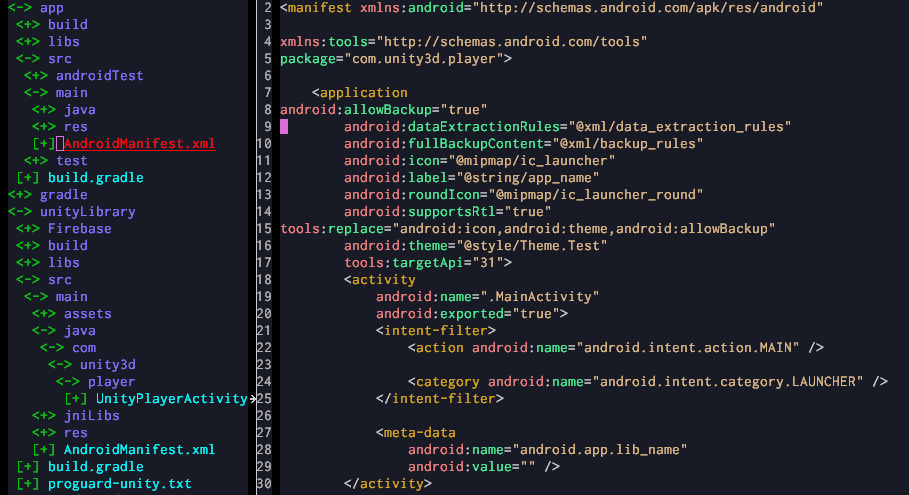
\includegraphics[width=.9\linewidth]{./pic/unityToAndroid_20221123_223757.png}

\subsection{在app的build.gradle里加入这行代码。}
\label{sec-3-3}
\begin{minted}[fontsize=\scriptsize,linenos=false]{xml}
ndk {
    abiFilters 'armeabi-v7a'
}
\end{minted}

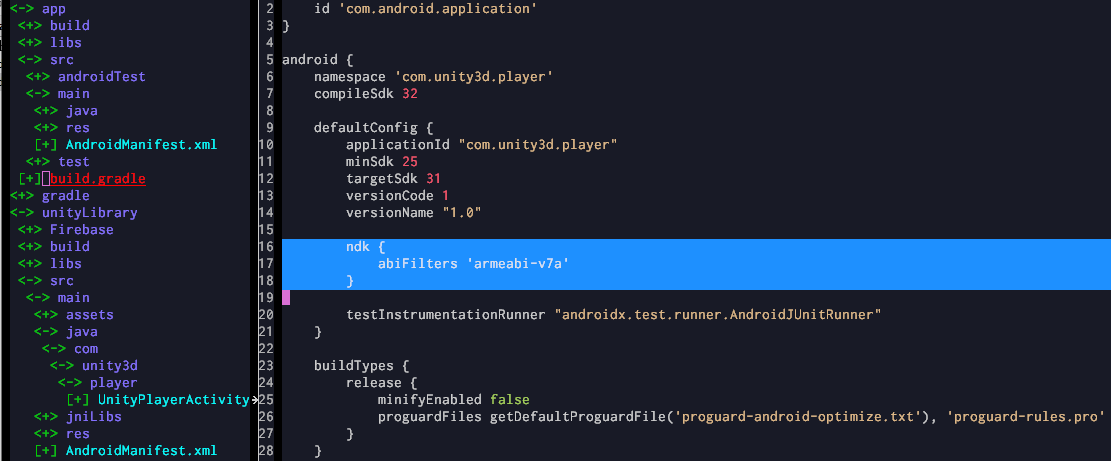
\includegraphics[width=.9\linewidth]{./pic/unityToAndroid_20221123_223842.png}
\subsection{在app的main->res->values->strings.xml里加入这行代码}
\label{sec-3-4}
\begin{itemize}
\item 都还没有去想,这句话能起到什么作用,应该是关系不大,或是可以跳过绕过的小细节
\begin{minted}[fontsize=\scriptsize,linenos=false]{xml}
<string name="game_view_content_description">Game view</string>
\end{minted}
\item 进行这两步操作的原因是,我在运行到手机时,他显示硬件不支持或者闪退。加入上面两个代码后就可以正常启动unity。
\item 我个人认为真正起作用的是上上一步关于手机架构的设置的ndk那三行,与上面字符串无关,应该是无关的
\end{itemize}

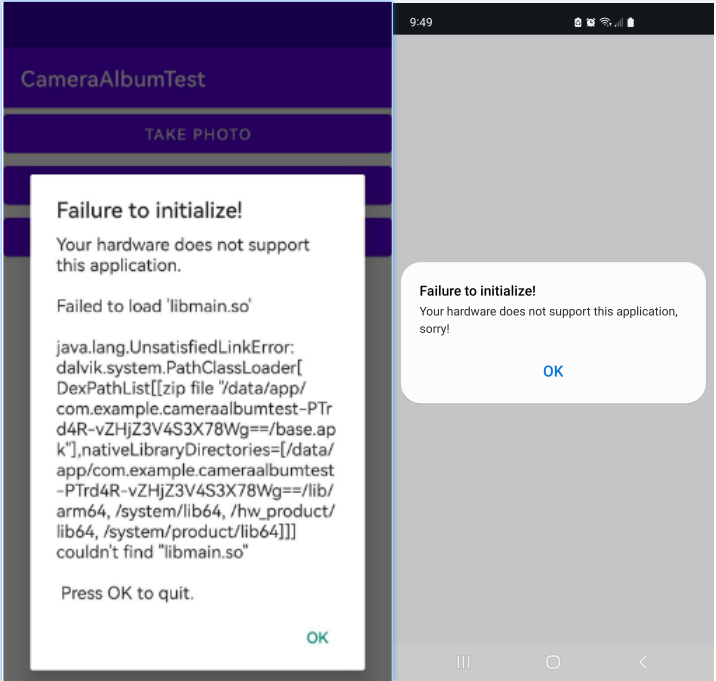
\includegraphics[width=.9\linewidth]{./pic/unityToAndroid_20221123_225409.png}

\subsection{点击按钮启动unity(画蛇添足)}
\label{sec-3-5}
\begin{itemize}
\item 感觉这个连接过程对于自己的项目就是画蛇添足.可是如何既能避开这一步,又能两者很好的平滑交互呢? 对于现在的自己,是个问题和挑战
\item 在主工程的activity\_main.xml 文件里添加一个按钮。MainActivity.java 里加入启动事件,如果在这里layout标红的话,就把鼠标移到layout下面,建立一个layout就行,我分析是主工程的问题,这个影响不大
\end{itemize}
\begin{minted}[fontsize=\scriptsize,linenos=false]{xml}
<Button
    android:id="@+id/showUnityBtn"
    android:layout_width="match_parent"
    android:layout_height="wrap_content"
    android:text="Show Unity"/>
\end{minted}

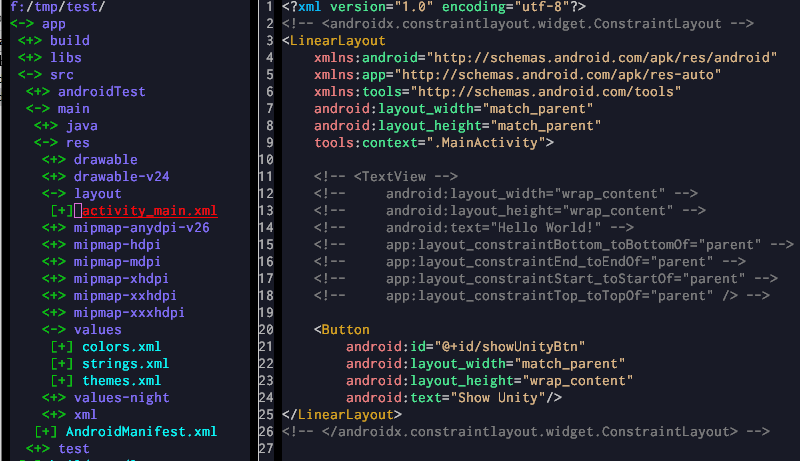
\includegraphics[width=.9\linewidth]{./pic/unityToAndroid_20221123_223751.png}
\begin{itemize}
\item MainActivity.cs 里的回调设置
\end{itemize}
\begin{minted}[fontsize=\scriptsize,linenos=false]{java}
Button btn = (Button)findViewById(R.id.showUnityBtn);
btn.setOnClickListener(new View.OnClickListener() {
        @Override
        public void onClick(View view) {

// <<<<<<<<<<<<<<<<<<<< UnityPlayerActivity <= com.unity3d.player 这里就是刚刚那个包名奇怪的地方,要不然 找不到 下面的 UnityPlayerActivity 类
            Intent intent = new Intent(MainActivity.this, UnityPlayerActivity.class); // <<<<<<<<<<<<<<<<<<<< UnityPlayerActivity

            startActivity(intent);
        }
    });
\end{minted}

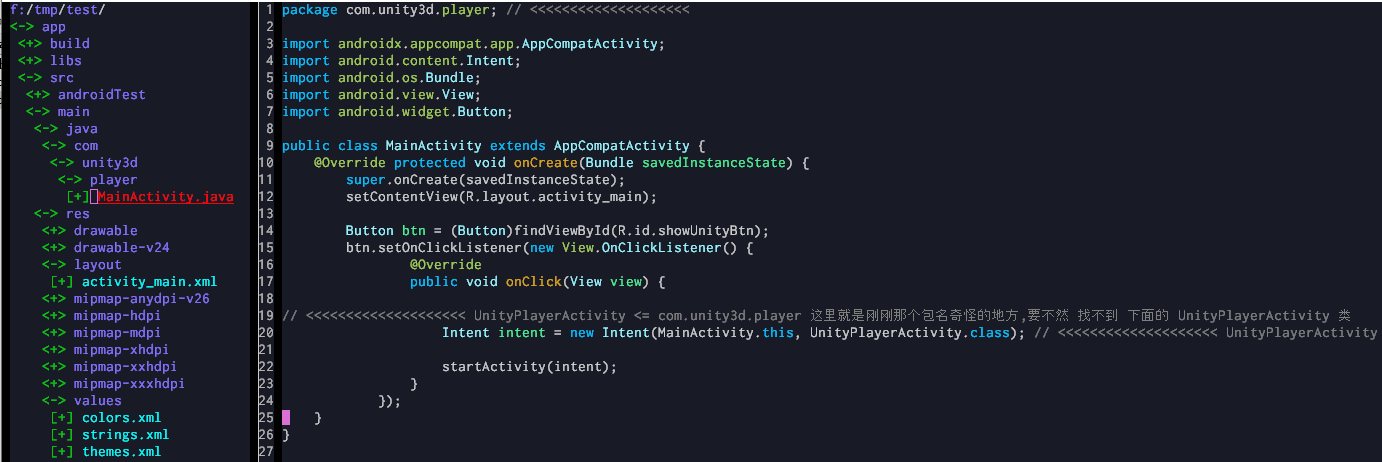
\includegraphics[width=.9\linewidth]{./pic/unityToAndroid_20221123_223852.png}
\subsection{在build.gradle中申明包裹类名称}
\label{sec-3-6}
\begin{itemize}
\item 说是现在在AndroidManifest.xml里申明包裹名称已经过时了,要在配置文件里申明,于是我在这里申明的:
\end{itemize}
\begin{minted}[fontsize=\scriptsize,linenos=false]{groovy}
android {
    namespace 'com.unity3d.player'
}
\end{minted}

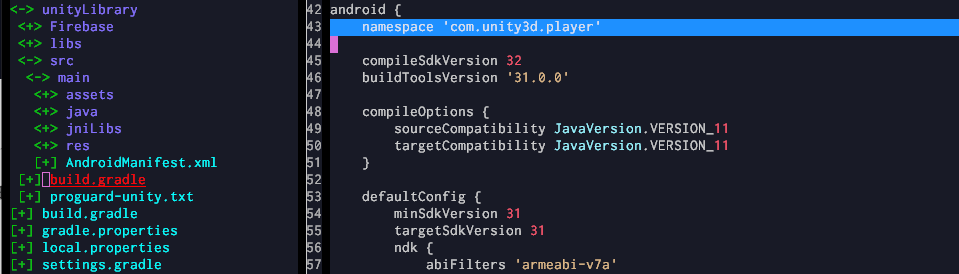
\includegraphics[width=.9\linewidth]{./pic/unityToAndroid_20221124_090438.png}

\section{启动运行}
\label{sec-4}

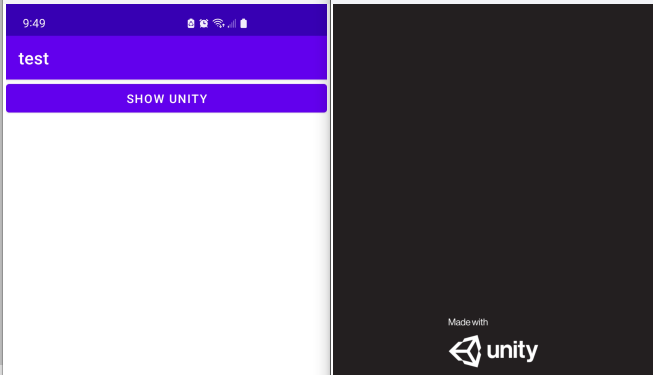
\includegraphics[width=.9\linewidth]{./pic/unityToAndroid_20221123_225517.png}

\section{Android Studio 类库中重复类的修复}
\label{sec-5}

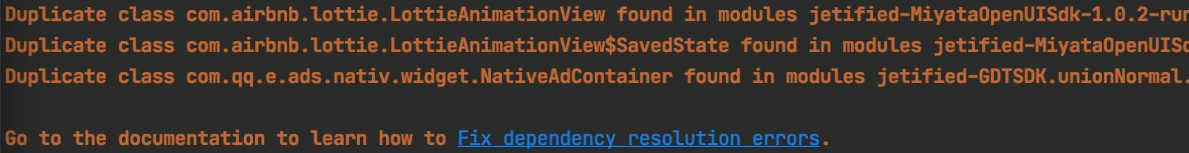
\includegraphics[width=.9\linewidth]{./pic/unityToAndroid_20221124_221720.png}
\begin{itemize}
\item 如果新导入的依赖库发生了 Duplicate class android.xx.xx 这种类型的报错可能就是两个库导入了重复的类,这时候只需要把build.gradle中新导入的依赖做如下处理
\begin{minted}[fontsize=\scriptsize,linenos=false]{xml}
implementation ('com.xxx.xxx.xx:xx:1.0.0'){
    exclude group: "com.xxxx.xxxx"
}
\end{minted}
\item 上面这个方法我还没有试.下面的试过了可行
\item 对,就是把新导入的依赖库的后面加上大括号并把重复导入包名填入相应的位置就可以解决了,有时候可能会好几个依赖库都重复了,这就比较难判断了
\item 1.把MiyataOpenUISdk-1.0.2.aar改后缀成zip,得到解压后的MiyataOpenUISdk-1.0.2文件夹,里面包含classes.jar和res等。
\end{itemize}

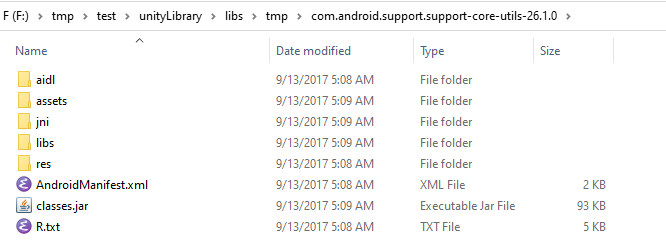
\includegraphics[width=.9\linewidth]{./pic/unityToAndroid_20221124_221954.png}
\begin{itemize}
\item 2.同理把classes.jar改后缀成zip,解压后得到classes文件夹,找到冲突的包,直接删除整个文件夹,如图
\item 3.使用jar命令重新对classes文件夹打包成jar ,并替换掉之前的classes.jar。
\end{itemize}
\begin{minted}[fontsize=\scriptsize,linenos=false]{shell}
jar cvf classes.jar -C classes/ .
\end{minted}
\begin{itemize}
\item 4.同理,使用jar命令重新对MiyataOpenUISdk-1.0.2文件夹打包成aar ,得到的newMiyataOpenUISdk.aar即可使用。
\end{itemize}
\begin{minted}[fontsize=\scriptsize,linenos=false]{shell}
 jar cvf com.android.support.support-compat-26.1.0.aar -C com.android.support.support-compat-26.1.0/ .
\end{minted}

\section{那么现在就是说:安卓SDK与unity的交互与打包基本没有问题了}
\label{sec-6}
\begin{itemize}
\item 但对自己更大的挑战是:为什么unity里一个空物件挂载到热更新的过程,我打包之后在安卓手机上运行不出来,仍需要时间debug这个过程
\item 过程中遇到过,还会遇到很多不懂的问题,比如同样的某些android studio里加android:exported="true"各种标签等,如果只用unity打包,该如何实现呢?两套不同的打包机制都得弄明白.但都是这么一个学习的过程,不会被轻易挫败.
\item 相比之下,安卓SDK的实现极其简单,可以放在后面,等这些疑难杂症都解决放心了,再去写简单一点儿的
\end{itemize}
\subsection{FATAL EXCEPTION: main}
\label{sec-6-1}

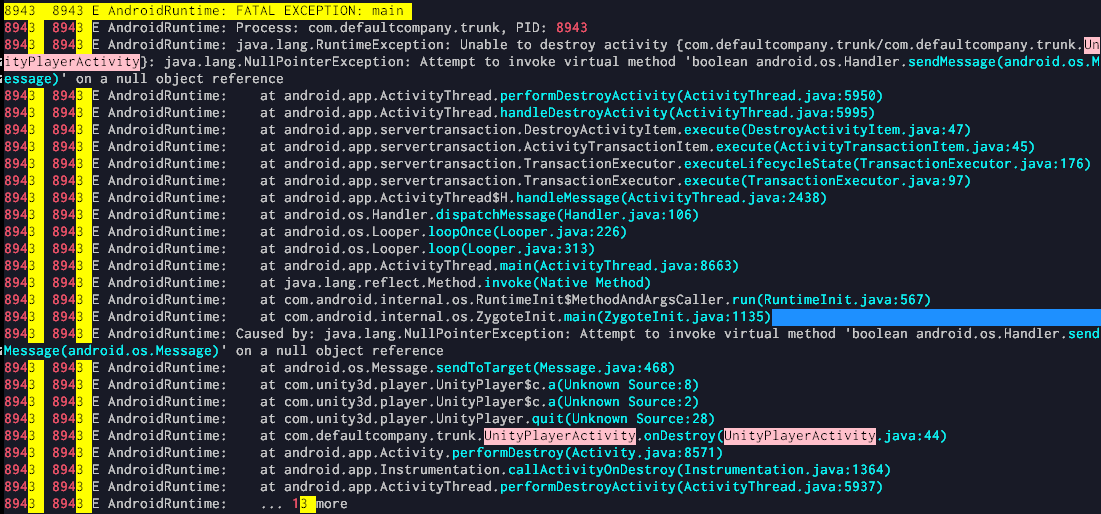
\includegraphics[width=.9\linewidth]{./pic/unityToAndroid_20221124_101807.png}
\begin{itemize}
\item 这个没有再出现了,根据这里改的:\url{https://forum.unity.com/threads/android-crashes-after-update-project-to-unity-2020-3-9f.1126979/}
\item 但是游戏的界面仍然是渲染不出来,还在找原因
\end{itemize}
\begin{minted}[fontsize=\scriptsize,linenos=false]{java}
@Override protected void onDestroy () {
    Log.d(TAG, "onDestroy() ");
    // mUnityPlayer.destroy();
    mUnityPlayer.removeAllViews();
    mUnityPlayer.quit();
    super.onDestroy();
}
\end{minted}
\subsection{安卓Android Studio库包中有依赖的库包的解决方案 7.2.2}
\label{sec-6-2}
\begin{minted}[fontsize=\scriptsize,linenos=false]{tex}
Direct local .aar file dependencies are not supported when building an AAR.
\end{minted}
\begin{itemize}
\item 在高版本的AndroidStudio并且使用了版本的gradle出现了上述问题可以按着如下引用
\end{itemize}
\subsubsection{在你工程根目录下新建一个文件夹 \textbf{unitylibs} ,将你的aar文件放入,然后在该目录下新建一个build.gradle文件}
\label{sec-6-2-1}

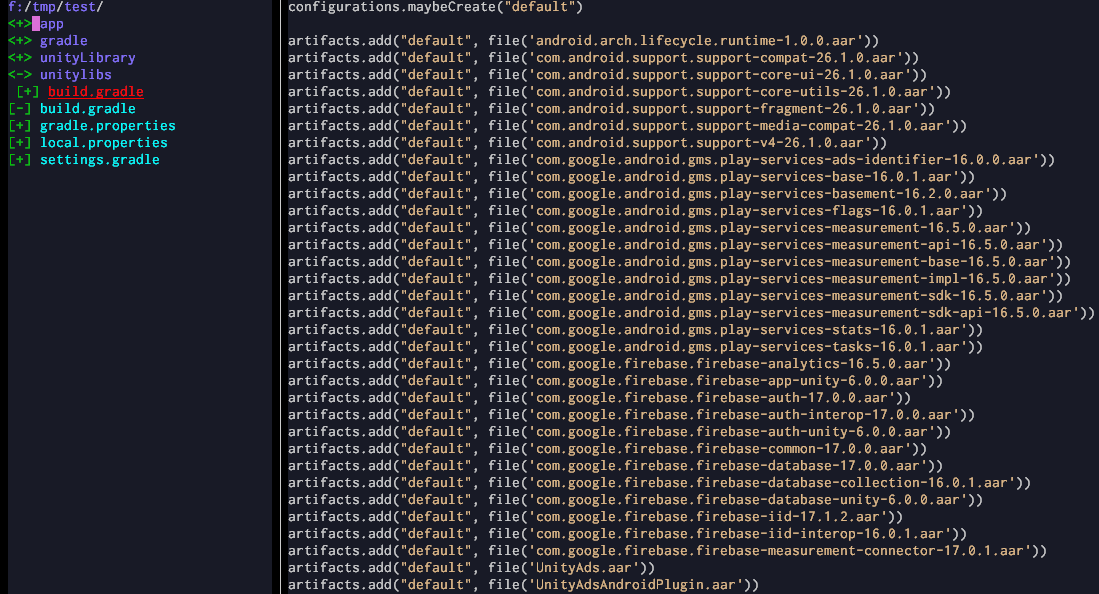
\includegraphics[width=.9\linewidth]{./pic/unityToAndroid_20221124_161335.png}
\subsubsection{在settings.gradle 导入该工程}
\label{sec-6-2-2}
\begin{minted}[fontsize=\scriptsize,linenos=false]{xml}
include ':unitylibs
\end{minted}

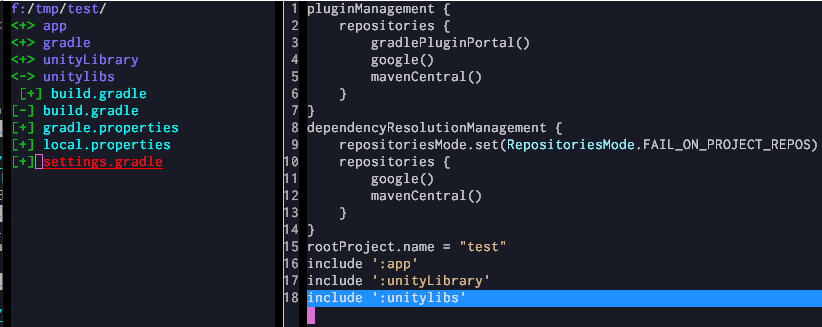
\includegraphics[width=.9\linewidth]{./pic/unityToAndroid_20221124_161424.png}
\subsubsection{在你需要依赖的工程里面的build.gradle中增加依赖}
\label{sec-6-2-3}
\begin{itemize}
\item // 这里需要注意的是,unitylibs是你aar库所在文件夹
\begin{minted}[fontsize=\scriptsize,linenos=false]{xml}
implementation project(path: ':unitylibs')
\end{minted}
\end{itemize}

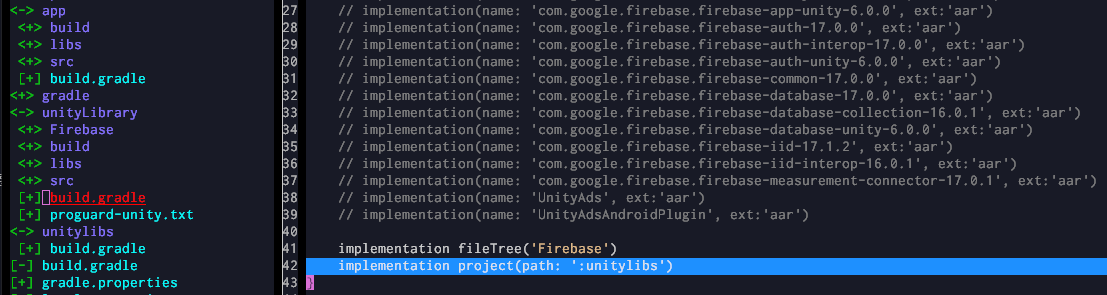
\includegraphics[width=.9\linewidth]{./pic/unityToAndroid_20221124_162337.png}
\begin{itemize}
\item 当然如果你有很多aar库,那么你需要在根目录创建一个LocalRepo目录,然后将你不同的aar库放在不同文件夹下。在setting.gradle分别导入
\item 下面它是这么说的,可是我都把它们放在同一个类库里,看不行的话再移.为什么每个包都需要一个单独的类库呢?解偶多个不同包之间的依赖性?加载时的内存性能影响等?
\end{itemize}

\subsection{类库包里的错误的修复问题}
\label{sec-6-3}
\begin{itemize}
\item 现在还不是很懂,或是还没有经历狠好地锻炼怎么改类库包里的错误,晚点儿再理会这些
\end{itemize}

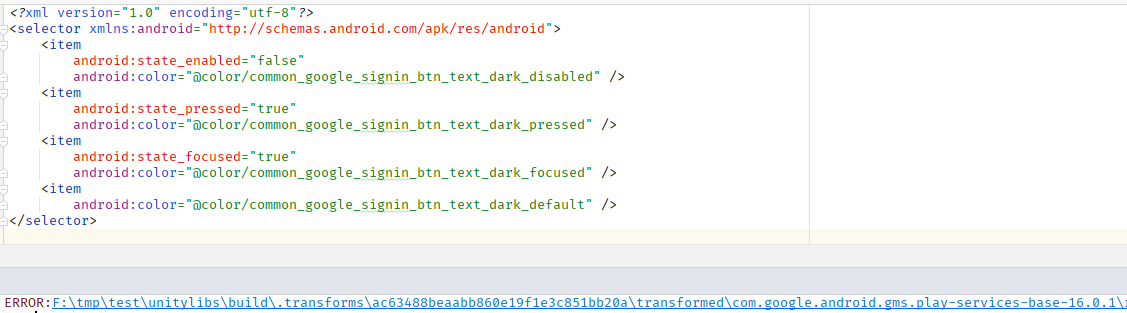
\includegraphics[width=.9\linewidth]{./pic/unityToAndroid_20221124_163004.png}
\begin{itemize}
\item 先只把这些有错误的类库包不连上
\end{itemize}

\section{安卓设备上资源包的存放位置,以及是否本地存放有需要的资源包}
\label{sec-7}

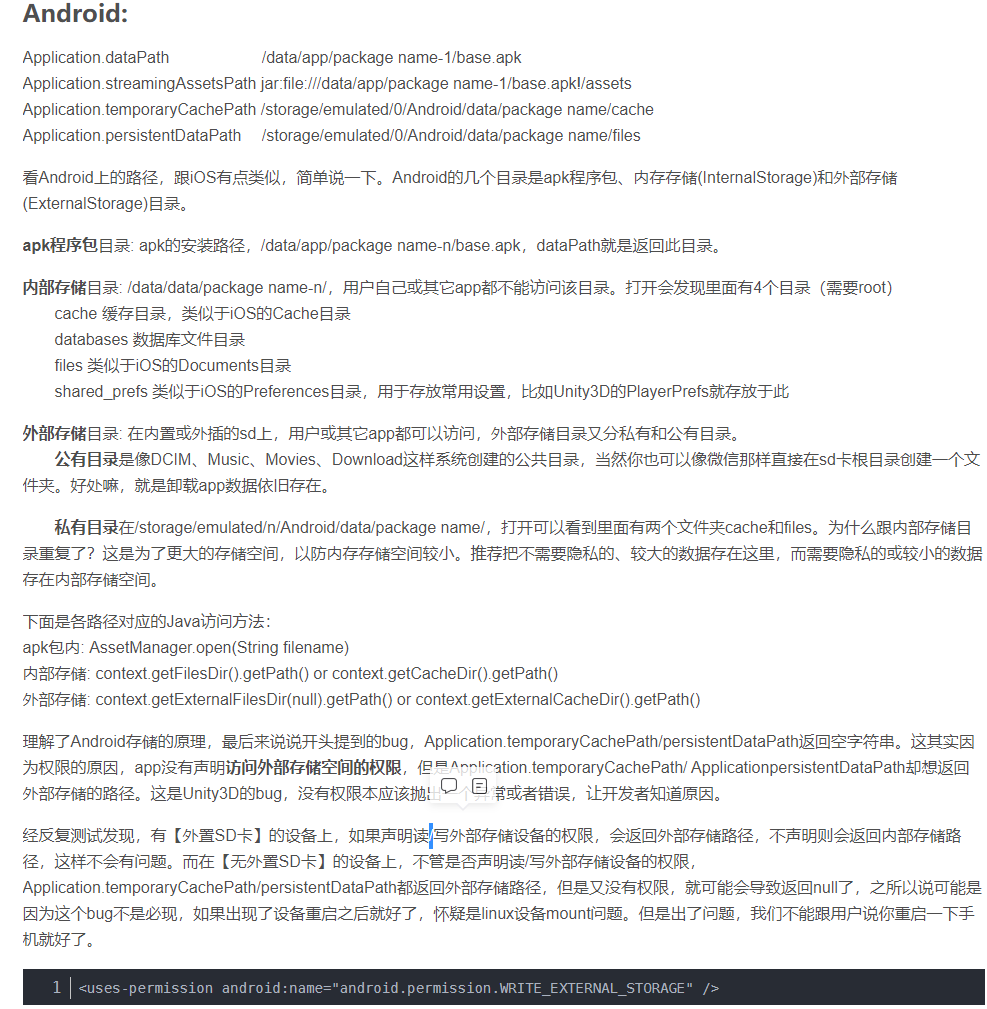
\includegraphics[width=.9\linewidth]{./pic/unityToAndroid_20221124_135846.png}

\begin{minted}[fontsize=\scriptsize,linenos=false]{tex}
Application.dataPath             /data/app/package name-1/base.apk
Application.streamingAssetsPath jar:file:///data/app/package name-1/base.apk!/assets
Application.temporaryCachePath  /storage/emulated/0/Android/data/package name/cache
Application.persistentDataPath  /storage/emulated/0/Android/data/package name/files
\end{minted}
\begin{itemize}
\item 看Android上的路径,跟iOS有点类似,简单说一下。Android的几个目录是apk程序包、内存存储(InternalStorage)和外部存储(ExternalStorage)目录。
\item \textbf{apk程序包目录}: apk的安装路径,/data/app/package name-n/base.apk,dataPath就是返回此目录。
\item \textbf{内部存储目录}: /data/data/package name-n/,用户自己或其它app都不能访问该目录。打开会发现里面有4个目录(需要root)
\item     cache 缓存目录,类似于iOS的Cache目录
\item     databases 数据库文件目录
\item     files 类似于iOS的Documents目录
\item     shared\_prefs 类似于iOS的Preferences目录,用于存放常用设置,比如Unity3D的PlayerPrefs就存放于此
\item 外部存储目录: 在内置或外插的sd上,用户或其它app都可以访问,外部存储目录又分私有和公有目录。
\item     公有目录是像DCIM、Music、Movies、Download这样系统创建的公共目录,当然你也可以像微信那样直接在sd卡根目录创建一个文件夹。好处嘛,就是卸载app数据依旧存在。
\item     私有目录在/storage/emulated/n/Android/data/package name/,打开可以看到里面有两个文件夹cache和files。为什么跟内部存储目录重复了?这是为了更大的存储空间,以防内存存储空间较小。推荐把不需要隐私的、较大的数据存在这里,而需要隐私的或较小的数据存在内部存储空间。
\item 下面是各路径对应的Java访问方法:
\begin{itemize}
\item apk包内: AssetManager.open(String filename)
\item 内部存储: context.getFilesDir().getPath() or context.getCacheDir().getPath()
\item 外部存储: context.getExternalFilesDir(null).getPath() or context.getExternalCacheDir().getPath()
\end{itemize}
\end{itemize}
理解了Android存储的原理,最后来说说开头提到的bug,Application.temporaryCachePath/persistentDataPath返回空字符串。这其实因为权限的原因,app没有声明访问外部存储空间的权限,但是Application.temporaryCachePath/ ApplicationpersistentDataPath却想返回外部存储的路径。这是Unity3D的bug,没有权限本应该抛出一个异常或者错误,让开发者知道原因。
\begin{itemize}
\item 经反复测试发现,有【外置SD卡】的设备上,如果声明读/写外部存储设备的权限,会返回外部存储路径,不声明则会返回内部存储路径,这样不会有问题。而在【无外置SD卡】的设备上,不管是否声明读/写外部存储设备的权限,Application.temporaryCachePath/persistentDataPath都返回外部存储路径,但是又没有权限,就可能会导致返回null了,之所以说可能是因为这个bug不是必现,如果出现了设备重启之后就好了,怀疑是linux设备mount问题。但是出了问题,我们不能跟用户说你重启一下手机就好了。
\end{itemize}
\begin{minted}[fontsize=\scriptsize,linenos=false]{xml}
<uses-permission android:name="android.permission.WRITE_EXTERNAL_STORAGE"/>
\end{minted}
% Emacs 27.2 (Org mode 8.2.7c)
\end{document}